\clearpage
\section{Original-device spatial gas coupling on native ceramic meshes}
The original 0.40\,$\times$\,0.40\,$\times$\,0.50 mm, 88-leg reference is retained. In each of the three interstage gaps, source-derived unobstructed rectangular columns were intersected with both native ceramic triangular surface meshes. The common refinement contains 752 columns and 6109 intersection polygons. Exact polygon area and linear P1 shape-function integrals distribute equal and opposite gas heat to the original tetrahedral ceramic nodes; the nonlinear gas flux itself uses one centroid evaluation per intersection polygon. This is a spatial reduced model, not a gas-domain field solution.

\begin{table}[htbp]
\centering
\caption{Area of paired, unobstructed bare-ceramic source regions. Both surfaces of each pair are covered by the same common-refinement area.}
\begin{tabular}{lrr}
\toprule
Gap & Paired area (mm$^2$) & Area error (mm$^2$) \\
\midrule
C0--C1 & 7.428064 & $-1.8\times10^{-15}$ \\
C1--C2 & 5.497517 & $+1.8\times10^{-15}$ \\
C2--C3 & 1.979438 & $-4.4\times10^{-16}$ \\
\bottomrule
\end{tabular}
\end{table}

For an explicitly conditional original-device case, the previous exterior and interstage gas proxies were disabled; the selected bare-ceramic columns provide the only gas exchange, all other gas boundaries are adiabatic, and gray radiation remains a separate process. At 300 K bath, 100 Pa krypton, accommodation 0.8, 2 mW die heat and 0.595668 W electrical input, the coupled calculation gives 218.659107 K die temperature, 218.591711 K top ceramic, 303.744877 K hot ceramic, 0.399961 A and 1.489316 V. The three gas-link heat flows are 2.534996, 1.197643 and 0.511544 mW. Maximum independent stage and global energy residuals are $1.06\times10^{-9}$ W and $9.15\times10^{-10}$ W. The previous 219.368939 K result used different overlapping gas proxies; the $-0.709832$ K difference combines omitted and redistributed gas paths and is not a prediction of physical improvement.

\begin{figure}[htbp]
\centering
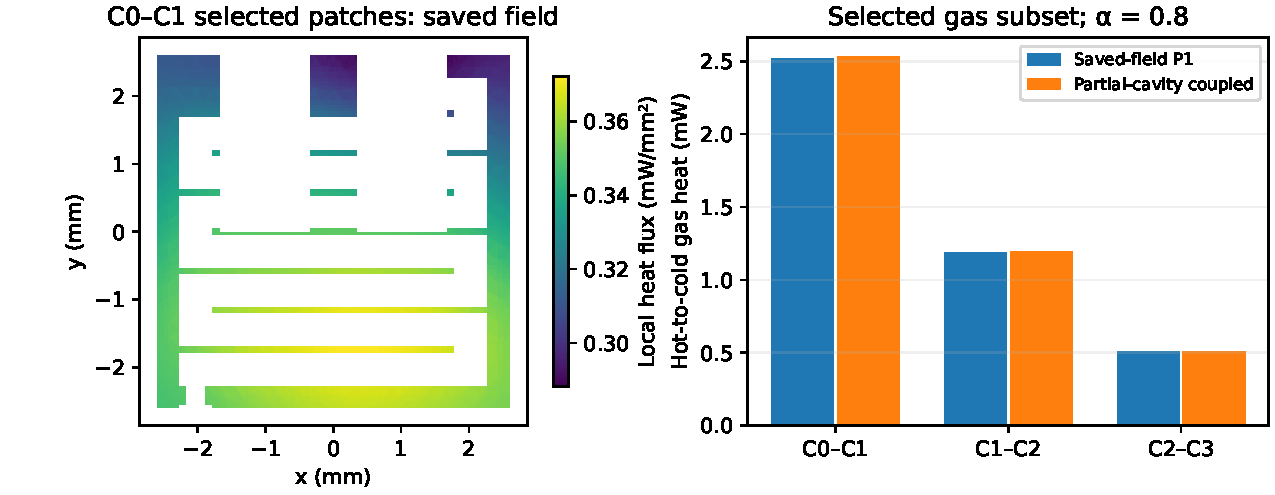
\includegraphics[width=0.96\textwidth]{figures/v325_nominal_p1_gas.pdf}
\caption{Source-mesh P1 gas exchange over selected bare-ceramic patches and gap heat flows. White areas are not represented gas-exchange surfaces. The saved-field diagnostic and conditional coupled result use the same geometry and assumed accommodation.}
\end{figure}

The paired surface area totals 29.810036 mm$^2$, 3.3004\% of the registered gas-facing area. Six faces are partly covered; 1834 faces have no P1 patch and 173 temperature-proxy assignments remain unresolved. Patterned metal, lead and enclosure transport are not completed. Krypton conductivity and temperature-jump parameters are assumptions; the coupled result is neither a complete cavity solution nor experimental validation. Native metal electrical current-flux qualification and the historical bath, cold-interface and gas-flux gates remain failed.
